124. \begin{figure}[ht!]
\center{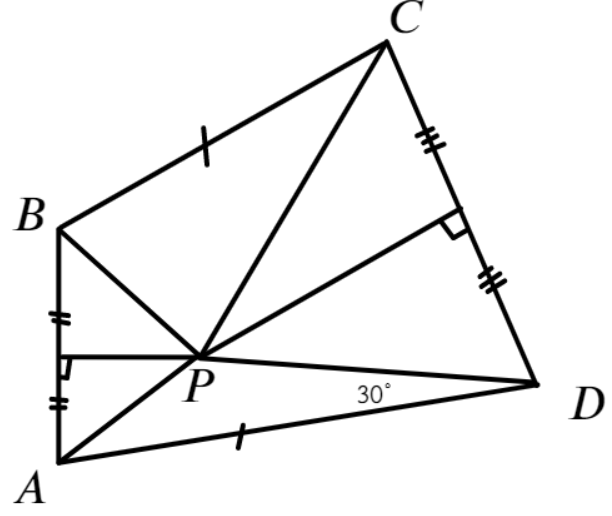
\includegraphics[scale=0.35]{g8-124.png}}
\end{figure}\\
В треугольниках $ABP$ и $DCP$ медиана совпадает с высотой, значит они равнобедренные и $AP=BP,\ DP=CP.$ Тогда треугольники $APD$ и $BPC$ равны по трём сторонам ($AP=BP,\ DP=CP,\ BC=AD,$ значит $\angle BCP=\angle ADP=30^\circ.$\\
